% Template: tam giác nhọn ABC nội tiếp đường tròn (O), có 3 đường cao + trực tâm H.
% Cách chỉnh:
%   - Đổi vị trí A, B, C bằng góc cực để có hình ưng ý.
%   - Thêm/xoá đối tượng phụ trợ trong các block "Đối tượng phụ trợ" và "Đối tượng nhấn".
\documentclass[border=5pt]{standalone}
\usepackage{tikz}
\usetikzlibrary{calc,intersections,through,angles,quotes}
\begin{document}
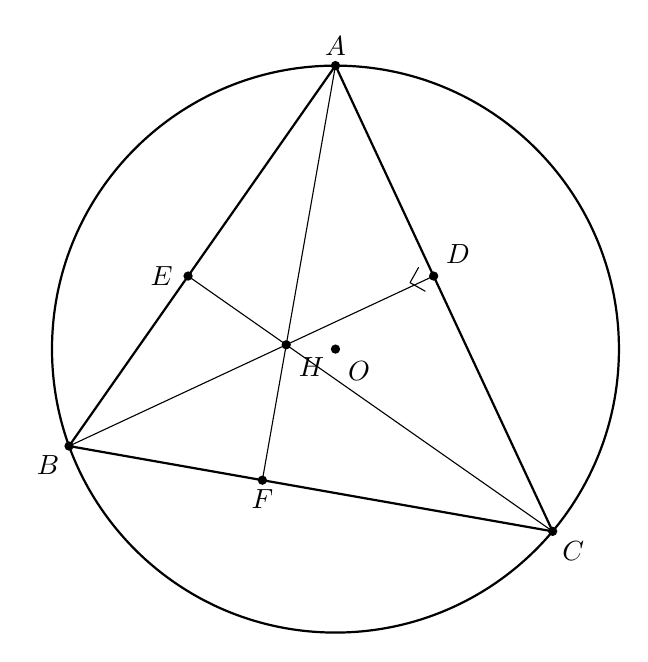
\begin{tikzpicture}[scale=1.2, line cap=round, line join=round]
  % --- Toạ độ ---
  \coordinate (O) at (0,0);
  \coordinate (A) at (90:3);
  \coordinate (B) at (200:3);
  \coordinate (C) at (-40:3);
  % chân đường cao
  \coordinate (D) at ($(A)!(B)!(C)$);   % chân đường cao từ B xuống AC
  \coordinate (E) at ($(A)!(C)!(B)$);   % chân đường cao từ C xuống AB
  \coordinate (F) at ($(B)!(A)!(C)$);   % chân đường cao từ A xuống BC
  % trực tâm = giao 2 đường cao
  \coordinate (H) at (intersection of B--D and C--E);

  % --- Đường tròn (O) và tam giác ABC ---
  \draw[thick] (O) circle (3);
  \draw[thick] (A) -- (B) -- (C) -- cycle;

  % --- Ba đường cao ---
  \draw (A) -- (F);
  \draw (B) -- (D);
  \draw (C) -- (E);

  % --- Ký hiệu góc vuông tại các chân đường cao (tuỳ chọn) ---
  % (cần điều chỉnh hướng tuỳ theo hướng đường cao; mẫu này vẽ tại D)
  \draw ($(D)+(-0.16,0.09)$) -- ($(D)+(-0.25,-0.07)$) -- ($(D)+(-0.09,-0.16)$);

  % --- Chấm điểm ---
  \foreach \p in {O,A,B,C,D,E,F,H} \fill (\p) circle (1.4pt);

  % --- Nhãn ---
  \node[above] at (A) {$A$};
  \node[below left] at (B) {$B$};
  \node[below right] at (C) {$C$};
  \node[above right=1pt] at (D) {$D$};
  \node[left=2pt] at (E) {$E$};
  \node[below] at (F) {$F$};
  \node[below right=1pt] at (H) {$H$};
  \node[below right=1pt] at (O) {$O$};
\end{tikzpicture}
\end{document}
